% Set up Document Format
\documentclass{article}

% Include packages for eps figures and math mode stuff (fonts and theorems)
\usepackage{epsfig}
\usepackage{amsfonts}
\usepackage{amsmath}

% Change Margins: This gives margins with 1in on top,
% .75 in on bottom and .75in on each side.
\textheight 9.25in
\textwidth 7in
\topmargin -.57in
\oddsidemargin -.25in
\evensidemargin -.25in

% Set up commands
\newtheorem{defin}{Definition}
\newtheorem{lemma}{Lemma}
\newtheorem{theorem}{Theorem}
\newcommand{\field}[1]{\mathbb{#1}}
\newcommand{\R}{\field{R}}
\newcommand{\C}{\field{C}}

\newcommand{\D}{\Delta}
\newcommand{\Dtry}{\Delta_{try}}
\newcommand{\DR}{\D_R}
\newcommand{\DRtry}{\D_{R,try}}
\newcommand{\DC}{\D_C}
\newcommand{\DCtry}{\D_{C,try}}
\newcommand{\DSet}{\mathbf{\Delta}}
\newcommand{\DRSet}{{\DSet_R}}
\newcommand{\DCSet}{{\DSet_C}}
\newcommand{\BDSet}{B_\DSet}
\newcommand{\BDRSet}{B_\DRSet}
\newcommand{\BDCSet}{B_\DCSet}

\newcommand{\bmtx}[1]{\left[\begin{array}{#1}}
\newcommand{\emtx}{\end{array}\right]}
\newcommand{\bsmtx}{\left[ \begin{smallmatrix}}
\newcommand{\esmtx}{\end{smallmatrix} \right]}
\newcommand{\be}{\begin{equation}}
\newcommand{\ee}{\end{equation}}

\newcommand{\maxsv}[1]{\bar{\sigma}\left(#1 \right)}
\newcommand{\minsv}[1]{\underline{\sigma}\left(#1\right)}

\providecommand{\e}[1]{\ensuremath{\times 10^{#1}}}

\begin{document}
%-------------------------------------------------------
%       Title/Author Information
%-------------------------------------------------------
\title{Multipoly: A Toolbox for Multivariable Polynomials \\ Version 2.01}
\author{Pete Seiler \\ \texttt{pseiler@umich.edu} \\[5mm] Sachin Shivakumar \\ \texttt{sshivak8@asu.edu}}
\date{\today}
\maketitle

%-------------------------------------------------------
%                       Abstract
%-------------------------------------------------------
\begin{abstract}

  Multipoly is a Matlab toolbox for the creation and manipulation of
  polynomials with one or more variables.  This document briefly
  describes the use and functionality of this toolbox.
  Section~\ref{sec:install} describes the installation of the toolbox.
  Section~\ref{sec:basic} gives a brief introduction on the basic
  functionality of the toolbox. More advanced functionality is
  descrbied in Section~\ref{sec:advanced} shows more advanced
  functionality.  Full documentation for all toolbox functions is
  provided in Section~\ref{sec:fulldoc}.

\end{abstract}

%-------------------------------------------------------
%          Installation
%-------------------------------------------------------
\section{Installation}
\label{sec:install}

The toolbox was tested with MATLAB versions R2009a and R2009b.  The
multipoly objects have been constructed using Matlab's new object
oriented programming syntax. As a result, the toolbox will not
function correctly in R2007b and earlier versions of Matlab. To
install the toolbox:
\begin{itemize}
\item Download the zip file and extract the contents to the directory
  where you want to install the toolbox.
\item Add the mulitpoly directory to the Matlab path, e.g. using
  Matlab's \texttt{addpath} command.  Note that the toolbox will not
  work if you are currently in the @polynomial directory.  This is due
  to MATLAB’s handling of object methods.
\item As described below, the \texttt{subs} command can be used to
  evaluate polynomials at specific values of the variables.  The
  toolbox contains one lower level mex function, \texttt{peval.c},
  which can be compiled to greatly speed up evaluation of polynomials.
  To compile this mex file, change to the
  multipoly$\backslash$@polynomial$\backslash$private folder.  Type
  \texttt{mex peval.c} in this folder to compile the mex function.
  There is a m-file version of this function which will be called if
  the mex version is not compiled but polynomial evaluations will be
  significantly slower than the compiled mex function.
\end{itemize}

%-------------------------------------------------------
%        Basic Functionality
%-------------------------------------------------------
\section{Basic Functionality}
\label{sec:basic}

Polynomial objects are most easily constructed by performing
basic operations on polynomial variables.  Use the \texttt{pvar}
command to create polynomial variables, e.g.

\begin{verbatim}
>> pvar x1 x2 x3
\end{verbatim}
A multivariable polynomial object can be created from these variables
using addition, multiplication, and exponentiation:

\begin{verbatim}
>> p = x3^4+5*x2+x1^2
p =
  x3^4 + x1^2 + 5*x2
\end{verbatim}
Matrices of polynomials can be created from polynomials using
horizontal/vertical concatenation and block diagonal augmentation:

\begin{verbatim}
>> p = x3^4+5*x2+x1^2
p =
  x3^4 + x1^2 + 5*x2

>> M1=[p 2*x2]
M1 =
  [ x3^4 + x1^2 + 5*x2 , 2*x2 ]

>> M2=[p; 2*x1*x2*x3]
M2 =
  [ x3^4 + x1^2 + 5*x2 ]
  [         2*x1*x2*x3 ]

>> M3 = blkdiag(p,x1-5)
M3 =
  [ x3^4 + x1^2 + 5*x2 ,      0 ]
  [                  0 , x1 - 5 ]
\end{verbatim}
Elements of a polynomial matrix can be referenced and assigned using
the standard MATLAB referencing notation:

\begin{verbatim}
>> M3
M3 =
  [ x3^4 + x1^2 + 5*x2 ,      0 ]
  [                  0 , x1 - 5 ]

>> M3(2,2)
ans =
  x1 - 5

>> M3(1,:)
ans =
  [ x3^4 + x1^2 + 5*x2 , 0 ]

>> M3(1,2) = (x1+2)^2
M3 =
  [ x3^4 + x1^2 + 5*x2 , x1^2 + 4*x1 + 4 ]
  [                  0 ,          x1 - 5 ]
\end{verbatim}


%-------------------------------------------------------
%          Advanced
%-------------------------------------------------------
\section{Advanced Functionality}
\label{sec:advanced}

This section describes some of the additional features of the
multipoly toolbox.  A complete list of implemented functions
can be found in Section~\ref{sec:fulldoc}.

\subsection{Creating Polynomials}


The toolbox contains several functions to construct polynomials of
specialized form. The \texttt{mpvar} function can be used to create a
polynomial matrix variable:

\begin{verbatim}
>> P = mpvar('p',[4 2])
P =
  [ p_1_1, p_1_2]
  [ p_2_1, p_2_2]
  [ p_3_1, p_3_2]
  [ p_4_1, p_4_2]

>> P = mpvar('p',[4 4],'s')
P =
  [ p_1_1, p_1_2, p_1_3, p_1_4]
  [ p_1_2, p_2_2, p_2_3, p_2_4]
  [ p_1_3, p_2_3, p_3_3, p_3_4]
  [ p_1_4, p_2_4, p_3_4, p_4_4]
\end{verbatim}
The first argument of \texttt{mpvar} specifies the prefix for the
variable names in the matrix and the the second argument specifies the
matrix size. The \texttt{'s'} option in the second example is used to
construct square, symmetric polynomial matrix variables.

The \texttt{monomials} function is used to construct a
vector list of monomials:
\begin{verbatim}
>> pvar x1 x2
>> Z1 = monomials([x1;x2],0:2)
Z1 =
  [     1]
  [    x1]
  [    x2]
  [  x1^2]
  [ x1*x2]
  [  x2^2]

\end{verbatim}
The first argument of \texttt{monomials} specifies the variables used
to construct the monomials vector.  The second argument specifies the
degrees of monomials to include in the monomials vector. In the
example above, the vector \texttt{Z1} returned by \texttt{monomials}
contains all monomials in variables \texttt{x1} and \texttt{x2} of
degrees 0,1, and 2.

The toolbox contains two functions to compute least squares
polynomial fits. \texttt{pdatafit} computes a polynomial fit to given
input/output data. \texttt{pfunctionfit} computes a polynomial
fit to a specified function. Syntax and examples for these functions
is provided in Section~\ref{sec:fulldoc}.

The toolbox also contains functions to convert between the multipoly
and symbolic toolboxes.  \texttt{s2p} converts from a polynomial from
a symbolic toolbox object to a multipoly object.  \texttt{p2s}
converts a polynomial from a multipoly to a symbolic object. The
two toolboxes have different functionality and it can be useful
to convert back and forth depending on the desired functionality.

Finally, it is possible to directly create a multivariable polynomial
by calling the \texttt{polynomial} constructor.  The data structure
used by the multipoly toolbox to represent polynomials must be
understood in order to use this constructor.  The coefficients,
monomials degrees, and variables names are stored for each polynomial.
A simple scalar example illustrates the data structure:

\begin{verbatim}
>> pvar x1 x2 x3
>> p = 3*x3^4+5*x2*x3+7*x1^2
p =
  3*x3^4 + 7*x1^2 + 5*x2*x3
>> full(p.coefficient)
ans =
     3
     7
     5
>> full(p.degmat)
ans =
     0     0     4
     2     0     0
     0     1     1
>> p.varname
ans =
    'x1'
    'x2'
    'x3'

\end{verbatim}

Each row of the degree matrix describes one term in the polynomial.
The columns of the degree matrix correspond to the listing of the
variables in \texttt{p.varname}.  In this example, the rows of the
degree matrix correspond to the monomials $x_3^4$, $x_1^2$, and
$x_2x_3$, respectively.  The rows of the coefficient matrix provide
the coefficients for the monomial specified by the corresponding row
of the degree matrix.  In this example, the rows of the coefficient
and degree matrices specify the terms $3x_3^4$, $7x_1^2$, and
$5x_2x_3$.


Next consider an $N\times M$ polynomial in $V$ variables consisting of
$T$ terms. This polynomial is stored as an $T\times NM$ sparse
coefficient matrix, a $T \times V$ degree matrix and a $V\times 1$
cell array of variable names. It might be more natural to represent
the coefficient matrix as an NxMxT array of coefficients. However,
MATLAB does not support 3D sparse arrays. To exploit sparsity, the
coefficient matrix is stored as an TxNM array. Below is an example
showing the data structure information for a polynomial matrix.

\begin{verbatim}
>> pvar x1 x2

>> M = [x1^2+7*x1*x2 -3*x1*x2; 0 2*x2+5]
M =
  [ x1^2 + 7*x1*x2, -3*x1*x2]
  [              0, 2*x2 + 5]

>> full(M.coefficient)
ans =
     1     0     0     0
     7     0    -3     0
     0     0     0     2
     0     0     0     5

>> full(M.degmat)
ans =
     2     0
     1     1
     0     1
     0     0

>> M.varname
ans =
    'x1'
    'x2'

>> M.matdim
ans =
     2     2
\end{verbatim}

The field \texttt{matdim} gives the dimensions of the matrix
polynomial. The rows of the degree matrix represent the four monomials
$x_1^2$, $x_1x_2$, $x_2$ and $1$. Each row of the coefficient matrix
can be reshaped into a $2\times 2$ coefficient matrix. For example,
the second row of the coefficient matrix is reshaped to:

\begin{verbatim}
full( reshape(M.coefficient(2,:),M.matdim) )
ans =
     7    -3
     0     0

\end{verbatim}

Thus the second row of the coefficient and degree matrices specifies
the term $\bsmtx 7 & -3 \\ 0 & 0 \esmtx x_1 x_2$.


The \texttt{polynomial} constructor directly constructs a polynomial
given the coefficient, monomial degree matrix, variable names, and
matrix dimensions.  The constructor synatx is:

\begin{verbatim}
P=polynomial(Coefficient,Degmat,Varname,Matdim)

\end{verbatim}


\subsection{Polynomial Manipulations}

The toolbox contains functions to easily manipulate and evaluate
polynomial expressions.  The \texttt{subs} function can be used
to replace polynomial variables with either symbolic or numeric
expressions.  A simple example is shown below:

\begin{verbatim}
>> pvar x1 x2 y1

>> x=[x1;x2];

>> p=2*x1^4+2*x1^3*x2-x1^2*x2^2+5*x2^4
p =
  2*x1^4 + 2*x1^3*x2 - x1^2*x2^2 + 5*x2^4

>> subs(p,x,[1;2])
ans =
  82

>> subs(p,x,[0 1 1; 1 0 2])
ans =
  [ 5, 2, 82]

>> subs(p,x,[y1;0])
ans =
  2*y1^4

\end{verbatim}

Numeric substitions, as in the first two examples of \texttt{subs} above,
are performed with the private function \texttt{peval}.  These substitutions
are performed much more efficiently if the mex version of \texttt{peval.c}
is compiled as described in Section~\ref{sec:install}.  The last example
of \texttt{subs} above demonstrates a symbolic substitution.

The are a variety of other functions to group polynomial terms.  The
\texttt{cleanpoly} remove terms based on value of coefficient and
degree. The \texttt{poly2basis} projects the polynomial coefficients
onto a basis of monomials.  The \texttt{collect} function collects
coefficients of specified variables monomials.  Finally, the
\texttt{monomials} function can also be used to extract all monomials
the exist in a polynomial.

\begin{verbatim}
>> pvar x1 x2;

>> p = [x1^2-9, 5*x1+3*x1*x2-4*x2^2];

>> cleanpoly(p,[],2)
ans =
  [ x1^2, 3*x1*x2 - 4*x2^2]

>> m = monomials(p)
m =
  [     1]
  [    x1]
  [  x1^2]
  [ x1*x2]
  [  x2^2]


>> R = [x1^2; x2^2];

>> [V,R,e] = poly2basis(p,R);

>> [V R]
ans =
  [ 1,  0, x1^2]
  [ 0, -4, x2^2]

>> e
e =
  [ -9, 3*x1*x2 + 5*x1]

\end{verbatim}

In the example above, the \texttt{cleanpoly} function retains only the
quadratic terms in the polynomial \texttt{p}.  The \texttt{monomials}
function extracts all monomials that exist in \texttt{p}.  The
\texttt{poly2basis} function projects the polynomial of \texttt{p}
onto the monomials listed in \texttt{R}.  Each row of \texttt{V}
provides the coefficients of the monomial in the corresponding row of
\texttt{R}.  In this example, the second row of \texttt{V} is $\bsmtx
0 & -4 \esmtx$ representing the coefficient of $x_2^2$ in \texttt{p}.
\texttt{poly2basis} also returns the difference between the input
polynomial \texttt{p} and the projection \texttt{R'*V}, i.e.
\texttt{e = p-R'*V}.


The toolbox contains functions \texttt{diff} and \texttt{jacobian} to
compute derivatives of a polynomial.  There are also functions
\texttt{pcontour} and \texttt{pcontour3} to plot 2d and 3d contours of
a polynomial.  Finally, there are functions to linearize
(\texttt{plinearize}), trim (\texttt{ptrim}), sample
(\texttt{psample}), and simulate (\texttt{psim}) polynomials.

\subsection{Simulink Interface}

\texttt{polylib.mdl} contains a Simulink block for polynomial objects.
A polynomial object and its input variables are specified in the
dialog box of the object.  The block output is the polynomial evaluated
at the input of this block.  This block can be used to integrate polynomial
objects into Simulink models.

%-------------------------------------------------------
% Acknowledgments
%-------------------------------------------------------
\section{Acknowledgments}

This research was partially supported under the NASA Langley NRA
contract NNH077ZEA001N entitled ``Analytical Validation Tools for Safety
Critical Systems'' and the NASA Langley NNX08AC65A contract
entitled 'Fault Diagnosis, Prognosis and Reliable Flight
Envelope Assessment.'' The technical contract monitors are Dr. Christine
Belcastro and Dr. Suresh Joshi, respectively.

%-------------------------------------------------------
%                REFERENCES (IN .BIB FILE)
%-------------------------------------------------------
%\bibliography{quasisos}

%-------------------------------------------------------
%          List of functions
%-------------------------------------------------------
\newpage
\section{List of Functions}
\label{sec:fulldoc}

The list of functions for polynomials is given below. This function
list can be displayed in Matlab by typing \texttt{help multipoly}.
The remainder of this section describes the purpose and syntax of most
polynomial functions.  This information can be displayed in Matlab by
typing \texttt{help functioname}.  Documentation for overloaded function
operations, e.g. \texttt{plus}, is not provided here but can be obtained
at the Matlab prompt using \texttt{help}.


\begin{verbatim}
Multivariate Polynomial Toolbox
  Version 2.00, 23 November 2010.

  Creating polynomial objects
     pvar         - Construct a polynomial variable
     mpvar        - Construct a matrix or vector polynomial variable
     polynomial   - Construct a polynomial object
     monomials    - Construct list of monomials
     pdatafit     - Compute a polynomial least squares fit to data
     pfunctionfit - Compute a polynomial least squares fit to a function

  Simulink:
     polylib.mdl  - Simulink block for polynomial objects

  Polynomial plotting:
     pcontour     - Plot 2d polynomial contours
     pcontour3    - Plot 3d polynomial contours

  Polynomial functions:
     poly2basis   - Project polynomial onto a basis of monomials
     plinearize   - Linearize a vector polynomial function
     ptrim        - Find trim conditions for a polynomial dynamical system
     psolve       - Find roots of a system of polynomials
     pvolume      - Estimate the volume of a polynomial set
     psample      - Draw random samples from a polynomial set
     psim         - Simulate a polynomial dynamical system
     pplanesim    - Plot the phase plane for a polynomial dynamical system
     int          - Element-by-element integration of a polynomial
     diff         - Element-by-element differentiation of a polynomial
     jacobian     - Compute Jacobian matrix of a polynomial vector
     collect      - Collect coefficients of specified variables
     subs         - Symbolic substitution
     cleanpoly    - Remove terms based on value of coefficient and degree

  Polynomial characteristics:
     isdouble     - True for arrays of doubles
     ispvar       - True for arrays of pvars
     ismonom      - True for arrays of monomials
     isempty      - True for empty monomials
     isequal      - Element by element polynomial comparisons
     size         - Size of a polynomial matrix
     length       - Length of a polynomial matrix
     fieldnames   - Get properties of a polynomial object

  Conversions:
     p2s          - Convert from multipoly to symbolic toolbox
     s2p          - Convert from symbolic toolbox to multipoly
     double       - Convert constant polynomial to a double
     char         - Converts a polynomial to its string representation.

  Overloaded arithmetic operations:
     plus, +      - Add polynomials
     minus, -     - Subtract polynomials
     mtimes, *    - Multiply polynomials
     mpower, ^    - Power of a polynomial
     horzcat, [,] - Horizontal concatentation of polynomials
     vertcat, [;] - Vertical concatentation of polynomials
     diag         - Diagonal poly matrices and diagonals of poly matrices
     tril         - Extract lower triangular part of a polynomial matrix
     triu         - Extract upper triangular part of a polynomial matrix
     blkdiag      - Block diagonal concatenation of polynomial matrices
     ctranspose, ' - Non-conjugate transpose of a polynomial
     transpose, .' - Non-conjugate transpose of a polynomial
     reshape      - Reshape a polynomial matrix
     repmat       - Replicate and tile an array of polynomials
     uplus        - Unary plus of a polynomial
     uminus       - Unary minus of a polynomial
     times, .*    - Element-by-element multiply of polynomials
     power, .^    - Element-by-element power of a polynomial
     sum          - Sum of the elements of a polynomial array
     prod         - Product of the elements of a polynomial array
     trace        - Sum of the diagonal elements
     det          - Determinant of a polynomial matrix
\end{verbatim}

%------------------------------------------------------------------------
\newpage
\subsection{PVAR}
\begin{verbatim}
function p = pvar(varargin)

  DESCRIPTION
    Create variables (i.e. monomials of degree 1).

  INPUTS
    X1,X2,...: Character strings used to name variables.

  OUTPUTS
    p: pvar

  SYNTAX
    pvar('x1','x2','x3')
    pvar x1 x2 x3
      Both of these function calls create monomials of degree 1 in the
      caller workspace with the given names. Any number of pvars can be
      created.
    p1 = pvar('x1')
      Creates a pvars named x1 and assigns it to the output variable p1.
    [p1,p2,...] = pvar('x1','x2',...)
      Creates many pvars and assigns them to the output variables.

  See also mpvar

\end{verbatim}

%------------------------------------------------------------------------
\newpage
\subsection{MPVAR}
\begin{verbatim}

function P = mpvar(cstr,N,M,opt);

  DESCRIPTION
    Create a polynomial matrix or vector variable

  INPUTS
    cstr: Character string to be used in creating the coefficient vector.
    N,M: row and column dimensions of polynomial matrix.
    opt: If N==M, then set opt = 's' to generate a symmetric
         matrix variable.

  OUTPUTS
    P: polynomial matrix

  SYNTAX
    P = mpvar('c',N)
        Creates an NxN polynomial matrix with entries c_i_j.
    P = mpvar('c',N,M)
    P = mpvar('c',[N,M])
        Creates an NxM polynomial matrix with entries c_i_j.
    P = mpvar('c',N,N,'s')
        Creates an NxN symmetric polynomial matrix with entries c_i_j.
    P = mpvar('c',[N,1])
    P = mpvar('c',[1,N])
        Creates an Nx1 or 1xN polynomial vector with entries c_i if
        N>1.  If N=1 then this creates a pvar named c.
    mpvar(cstr,N,M)
       Equivalent to calling eval([cstr '=mpvar(cstr,N,M);']).

  EXAMPLE
    P = mpvar('p',[2,3])

P =
  [ p_1_1, p_1_2, p_1_3]
  [ p_2_1, p_2_2, p_2_3]

  See also pvar


\end{verbatim}

%------------------------------------------------------------------------
\newpage
\subsection{POLYNOMIAL}
\begin{verbatim}
function P = polynomial(Coefficient,Degmat,Varname,Matdim);

  DESCRIPTION
    Creates a polynomial or a matrix of polynomials.

  INPUTS
    Coefficient: coefficients of each monomial.
    Degmat: degrees of each monomial
    Varname: names of variables
    Matdim: dimensions of the polynomial matrix

  OUTPUT
    P: polynomial object

  SYNTAX
    P=polynomial
      Creates an empty polynomial object.
    P=polynomial(Coefficient)
      If Coefficient is a real matrix of dimension NxM, then P is
      an NxM constant polynomial.
    P=polynomial(Varname)
      If Var is an NxM cell array of strings, then P is an NxM polynomial
      whose entries are the variables specified in Var.
    P=polynomial(Coefficient)
      If Coefficient is a polynomial object, then P=Coefficient.
    P=polynomial(Coefficient,Degmat,Varname,Matdim)
      If P is an NxM polynomial that is the sum of T terms in V
      variables, the inputs should be specified as:
        Coefficient is a Tx(N*M) sparse matrix.
           The coefficients of the (i,j) entry of the polynomial
           matrix are a Tx1 vector stored in the i+*N*(j-1) column of
           Coefficient.
        Degmat is a TxV sparse matrix of natural numbers.  Row t
           gives the degrees of each variable for the t^th term.
        Varname is a Vx1 cell array with entry v giving the name of
           variable v. For a constant polynomial, varname is an
           empty 1x1 cell.
        Matdim is a 1x2 vector of the matrix dimensions, [N M].


\end{verbatim}

%------------------------------------------------------------------------
\newpage
\subsection{MONOMIALS}
\begin{verbatim}

function Z=monomials(p,deg)

  DESCRIPTION
    Construct list of monomials

  INPUTS
    p: A polynomial, vector of pvars or a non-negative integer.
    deg: A vector of non-negative integers specifying the degrees
          of monomials to be included Z.

  OUTPUTS
    Z: lz-by-1 list of monomials

    Z: If p is a polynomial (deg is not specified) then Z will be a
       lz-by-1 vector of all monomials in p. If p is a vector of pvars
       then Z will be a lz-by-1 vector of all monomials of the specified
       degrees in the given pvars. If vars is a non-negative integer then
       Z will be the lz-by-var degree matrix with each row specifying the
       degrees of one of the monomials.

  SYNTAX
    Z=monomials(p)
       If p is a polynomial then Z is the vector of monomials in p.
    Z=monomials(vars,deg)
       If vars is a vector of pvars then Z is a vector of all monomials
       in the variables listed in vars and degrees listed in deg.
    Z=monomials(nvar,deg)
       If nvar is a non-negative integer then Z is the degree matrix
       corresponding to all monomials in nvar variables and degrees deg.

  EXAMPLE
    pvar x1 x2
    Z1 = monomials([x1;x2],0:2)

Z1 =
  [     1]
  [    x1]
  [    x2]
  [  x1^2]
  [ x1*x2]
  [  x2^2]

    p = x1^2+5*x1*x2-6*x2^3;
    Z2 = monomials(p)

Z2 =
  [  x1^2]
  [ x1*x2]
  [  x2^3]

  See also poly2basis


\end{verbatim}

%------------------------------------------------------------------------
\newpage
\subsection{PDATAFIT}
\begin{verbatim}
function [pfit,cfit,info] = pdatafit(p,x,Xdata,Ydata,W)

  DESCRIPTION
    This function finds the coefficients of a multivariate polynomial that
    best fits given data in a least-squares cost.  The data is fit
    with a linear combination of polynomial basis functions:
       p(x,c) = c1*f1(x)+c2*f2(x) + ... + ck*fk(x)
    where f1, f2, ..., fk are the polynomial basis functions. pdatafit
    computes the coefficients c1, c2, ..., ck that minimize the fitting
    error in a weighted squares cost:
       min_c  sum_i (W(i)*e(i))^2
    where e(i) is the fitting error of the i^th data point, i.e.
    e(i) := p(Xdata(i,:),c) - Ydata(i).

  INPUTS
    p: 1-by-1 polynomial.
    x: Nx-by-1 vector of pvars that specifies the independent variables
        in p.  All other variables in p are considered to be coefficients.
    Xdata: Nx-by-Npts matrix of input data values.  The i^th row of Xdata
        gives the data values associated with x(i).
    Ydata: 1-by-Npts vector of output data values
    W (Optional): 1-by-Npts weighting vector  [Default: W=ones(1,Npts)]

  OUTPUTS
    pfit: Least-squares polynomial fit
    cfit: Nc-by-2 cell array of the optimal coefficients.  The first
          column contains the coefficients (as chars) and the second
          column contains the optimal values.  The subs command can be
          be used to replace the coefficients in any polynomial with
          their optimal values, e.g. pfit = subs(p,cfit).
    info: Data structure containing the matrices in the least squares
          problem.  info has the fields A, b, cfit, W, e.  This gives
          the data of the least squares problem in the form:
                  min_c || diag(W)*(A*c-b) ||_2.
          e = A*cfit-b is the fitting error.

  SYNTAX
    [pfit,cfit,info] = pdatafit(p,x,Xdata,Ydata)
    [pfit,cfit,info] = pdatafit(p,x,Xdata,Ydata,W)

  EXAMPLE
   Xdata = linspace(100,200);
   Ydata = 1./Xdata;
   pvar c0 c1 c2 x;
   p=c0+c1*x+c2*x^2;
   [pfit,cfit,info] = pdatafit(p,x,Xdata,Ydata)
   plot(Xdata,Ydata,'bx',Xdata,double(subs(pfit,x,Xdata)),'r--')
   legend('1/X','pfit'); xlabel('x');

pfit =
  3.2808e-007*x^2 - 0.00014616*x + 0.0212
cfit =
    'c0'    [      0.0212]
    'c1'    [-1.4616e-004]
    'c2'    [ 3.2808e-007]
info =
       A: [100x3 double]
       b: [100x1 double]
    cfit: [3x1 double]
       W: [100x1 double]
       e: [100x1 double]

  See also pfunctionfit

\end{verbatim}

\begin{figure}[h]
\begin{center}
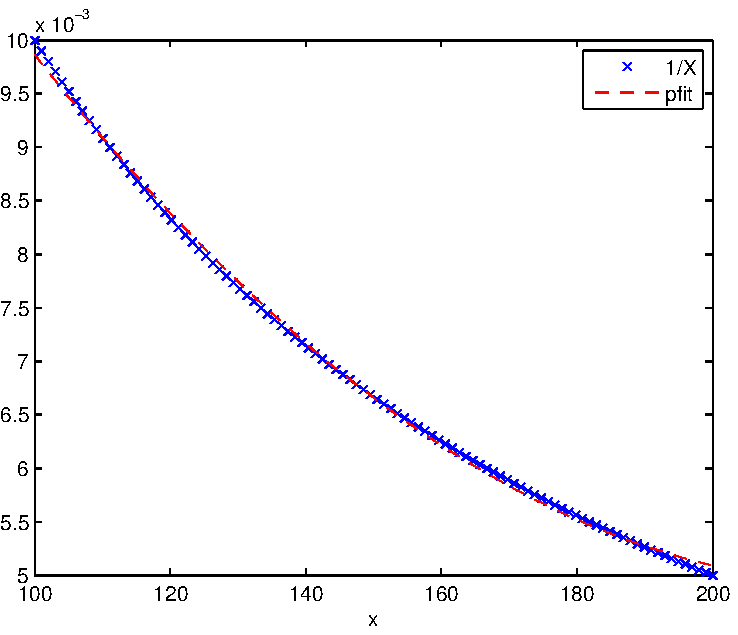
\includegraphics[width=4in]{figs/pdatafitPLOT.pdf}
\caption{Polynomial fit of $1/x$ using \texttt{pdatafit}}
\end{center}
\end{figure}

%------------------------------------------------------------------------
\newpage
\subsection{PFUNCTIONFIT}
\begin{verbatim}
function [pfit,cfit,fiterr] = pfunctionfit(p,x,Xdata,fnc,W)

  DESCRIPTION:
    This function finds the coefficients of a multivariate polynomial that
    best fits a function fnc in a least-squares cost.  The function is fit
    with a linear combination of polynomial basis functions:
       p(x,c) = c1*f1(x)+c2*f2(x) + ... + ck*fk(x)
    where f1, f2, ..., fk are the polynomial basis functions. pfunctionfit
    samples the function fnc and computes the coefficients c1, c2, ..., ck
    that minimize the fitting error on these samples in a weighted squares
    squares cost.  See pdatafit for more detail.

  INPUTS:
    p:     1-by-1 polynomial.
    x:     Nx-by-1 vector of pvars that specifies the independent variables
           in p.  All other variables in p are considered to be coefficients
    Xdata  (Optional): Nx-by-Npts  matrix of input data values at which to
           evaluate fnc for fitting. Alternatively, Xdata can be a
           structure with fields specying how to construct the data:
           fields to construct the Nvars-by-Npts input data set.
            - range:= Nx-by-2 matrix containing the data range [min max] of
              the variables defined in vars. Default is [-1 1]
            - sample:=defines the sampling technique. Choices are: 'grid',
              'uniform' ,'lhs'. Default is 'grid'. 'grid' generates
              linearly spaced data along each direction. 'uniform' draws
              random samples from the range using a uniform distribution.
              'lhs' uses the Latin Hypercube sampling technique. 'lhs'
               requires the Statistics Toolbox.
            - Npts: If sample='grid' then Npts is a Nvar-by-1 vector
              defining the number of points to be sampled along each
              direction. The total # of points is prod(Npts).  For 'lhs'
              or 'uniform', Npts is a 1-by-1 defining the total
              number of sampled points.
   fnc :   Function to fit with inputs x and 1-by-1 output. fnc can be
           a function handle, string expression, or polynomial.
   W (Optional): 1-by-Npts weighting vector .  Alternatively W can be
           a function handle, string expression, or polynomial.
           [Default: W=ones(1,Npts)]

  OUTPUTS:
    pfit: Least-squares polynomial fit
    cfit: Nc-by-2 cell array of the optimal coefficients.  The first
          column contains the coefficients (as chars) and the second
          column contains the optimal values.  The subs command can be
          be used to replace the coefficients in any polynomial with
          their optimal values, e.g. pfit = subs(p,cfit).
    info: Data structure containing the matrices in the least squares
          problem.  info has the fields A, b, cfit, W, e as described
          in pdatatfit help. It also contains Xdata and Ydata. Xdata are
          the input data samples and Ydata gives the values of fnc
          evaluated at Xdata. Sample information is stored in the fields
          sample, range, and Npts.

  SYNTAX
    [pfit,cfit,info] = pfunctionfit(p,vars,Xdata,fnc)
    [pfit,cfit,info] = pfunctionfit(p,vars,fnc)
    [pfit,cfit,info] = pfunctionfit(p,vars,Xdata,fnc,W)

  EXAMPLE
   fnc = @(x) sin(x);
   pvar c0 c1 c2 c3 x;
   vars = x;
   p = c0 + c1*x + c2*x^2 + c3*x^3;
   Xdata.sample ='uniform';
   Xdata.Npts = 20;
   [pfit,cfit,info] = pfunctionfit(p,vars,Xdata,fnc);
   ezplot(fnc,[info.range(1) info.range(2)]); hold on;
   xx = linspace(info.range(1),info.range(2),10);
   plot(xx,double(subs(pfit,vars,xx)),'r--'); hold off;
   legend('Original Function','Polynomial Fit'); xlabel('x');

  See also pdatafit, lhsdesign

\end{verbatim}

\begin{figure}[h]
\begin{center}
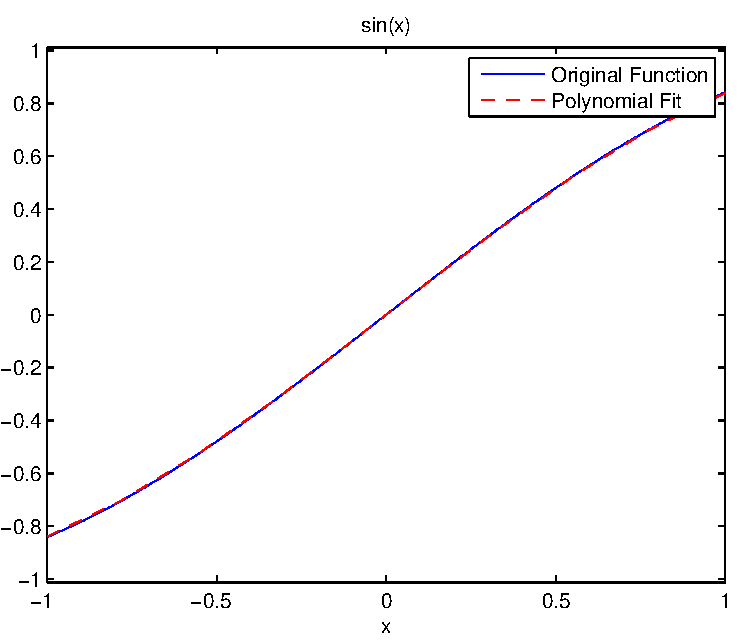
\includegraphics[width=4in]{figs/pfunctionfitPLOT.pdf}
\caption{Polynomial fit of $\sin(x)$ using \texttt{pfunctionfit}}
\end{center}
\end{figure}


%------------------------------------------------------------------------
\newpage
\subsection{POLYLIB}
\begin{verbatim}
POLYLIB.MDL  - Simulink block for polynomial objects

\end{verbatim}


\begin{figure}[h]
\begin{center}
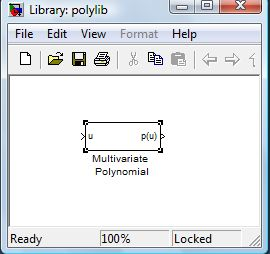
\includegraphics[height=3.0in]{figs/polylib.jpg}
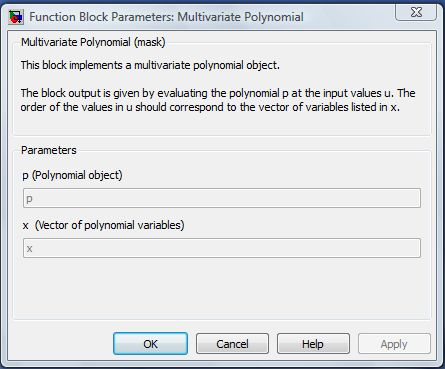
\includegraphics[height=3.0in]{figs/polylibdialog.jpg}
\caption{Polynomial Simulink Block (left) and dialog box (right)}
\end{center}
\end{figure}


%------------------------------------------------------------------------
\newpage
\subsection{PCONTOUR}
\begin{verbatim}
function [C,h] = pcontour(p,v,domain,linespec,npts,var)

  DESCRIPTION
    Plots contours of p(x,y) at the contour values specified by the vector
    v. The contours are generated numerically by evaluating p on a grid of
    values of x and y and then calling the CONTOUR function.

  INPUTS
    p: 1-by-1 polynomial of two variables
    v: N-by-1 vector of contour values (Default: v=1)
    domain: 1-by-4 vector specifying the plotting domain,
               [Xmin Xmax Ymin Ymax]
          (Default: domain = [-1 1 -1 1])
    linespec: Color and linetype.  (Default:  linespec='b')
    npts: 1-by-2 vector specifying the number of grid points along
           each axis, [Num of X pts, Num of Y pts]
           (Default: npts = [100 100])
    var: 1-by-2 vector of pvars specifying the x/y axis variables,
               [Variable for X axis, Variable for Y axis]
           (Default var = p.var)

  OUTPUTS
    C,h: Contour matrix and contour handle object returned by CONTOUR

  SYNTAX
   pcontour(p)
   pcontour(p,v)
   pcontour(p,v,domain)
   pcontour(p,v,domain,linespec)
   pcontour(p,v,domain,linespec,npts)
   pcontour(p,v,domain,linespec,npts,var)
   [C,h] = pcontour(p,v,domain,linespec,npts,var)

  EXAMPLE
   pvar x y
   p = (x-2)^2-(x-2)*y+y^2;
   domain = [0 4 -2 2];
   [C,h]=pcontour(p,[0.5 1 2],domain);
   clabel(C,h);

  See also contour, clabel, pcontour3

\end{verbatim}

\newpage
\begin{figure}[h]
\begin{center}
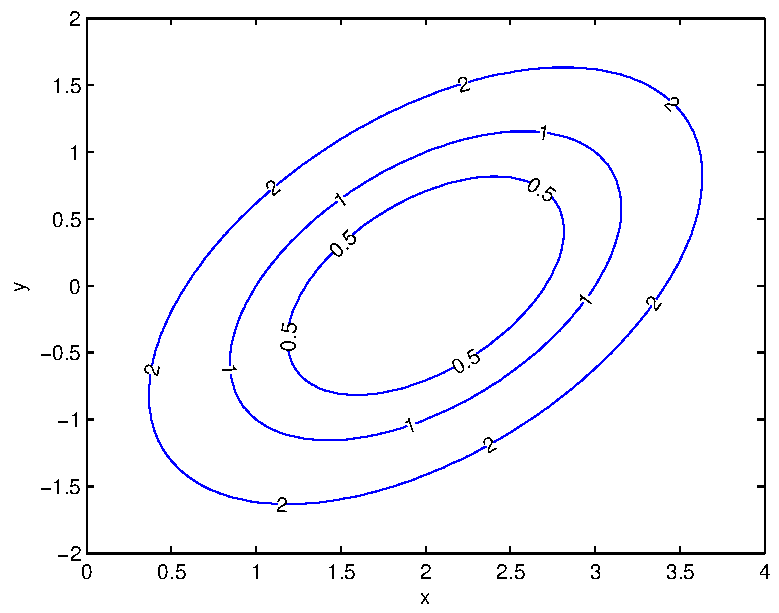
\includegraphics[width=4in]{figs/pcontourPLOT.pdf}
\caption{2-d contours of a quadratic polynomial using \texttt{pcontour}}
\end{center}
\end{figure}



%------------------------------------------------------------------------
\newpage
\subsection{PCONTOUR3}
\begin{verbatim}
function [F,V,C] = pcontour3(p,v,domain,npts,var)

  DESCRIPTION
    Plots contour surfaces of p(x,y,z) at the values specified by the
    vector v. The contours are generated numerically by evaluating p on a
    grid of values of x,y,z and then calling the ISOSURFACE function.

  INPUTS
    p: 1-by-1 polynomial of three variables
    v: N-by-1 vector of contour values (Default: v=1)
    domain: 1-by-6 vector specifying the plotting domain,
               [Xmin Xmax Ymin Ymax Zmin Zmax]
          (Default: domain = [-1 1 -1 1 -1 1])
    npts: 1-by-3 vector specifying the number of grid points along
           each axis, [Num of X pts, Num of Y pts, Num of Z pts]
           (Default: npts = [50 50 50])
    var: 1-by-3 vector of pvars specifying the x/y/z axis variables,
           [Variable for X axis, Variable for Y axis, Variable for Z axis]
           (Default var = p.var)

  OUTPUTS
    F,V,C: Faces, vertices, and facevertexcdata generated by ISOSURFACE.
          The 1,2, and 3 variable outputs are the same as those generated
          by ISOSURFACE.

  SYNTAX
   pcontour3(p)
   pcontour3(p,v)
   pcontour3(p,v,domain)
   pcontour3(p,v,domain,npts)
   pcontour3(p,v,domain,npts,var)
   [F,V,C] = pcontour3(p,v,domain,npts,var)

  EXAMPLE
   pvar x y z
   domain = [-3.5 3.5 -1.5 1.5 -1.5 1.5];
   p1 = x^2+y^2+z^2;
   ph1= patch(pcontour3(p1,2,domain));
   set(ph1, 'FaceColor', 'none', 'EdgeColor', 'red' );
   p2 = x^2/4+2*y^2+3*z^2;
   ph2= patch(pcontour3(p2,2,domain));
   set(ph2, 'FaceColor', 'blue', 'EdgeColor', 'none' );
   view(3); axis equal

  See also pcontour, isosurface

\end{verbatim}

\newpage
\begin{figure}[h]
\begin{center}
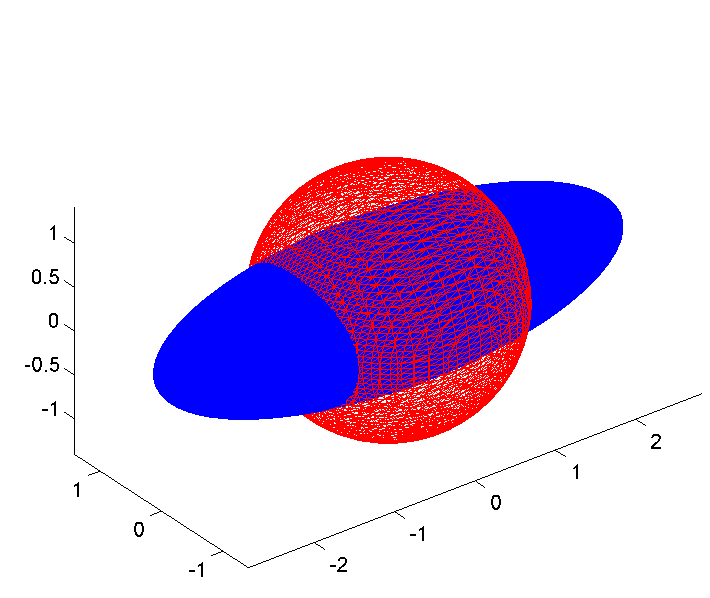
\includegraphics[width=4in]{figs/pcontour3PLOT.pdf}
\caption{3-d contours of quadratic polynomials using \texttt{pcontour3}}
\end{center}
\end{figure}


%------------------------------------------------------------------------
\newpage
\subsection{POLY2BASIS}
\begin{verbatim}
function [V,R,e] = poly2basis(p,R)

  DESCRIPTION
    Projects a vector of polynomials p onto the span of the monomials
    contained in the vector R.

  INPUTS
    p: 1-by-lp vector of polynomials.
    R [Optional]: lr-by-1 basis of monomials. [ Default: R=monomials(p) ]

  OUTPUTS
    V: lr-by-lp matrix expressing the projection of the polynomial p
       on the monomials in R. The projection of p on to the span of
       R is given by R'*V.
    R: Vector of monomials
    e: Difference between the input polynomial p and the projection
       R'*V, i.e. e = p-R'*V.  If R contains all monomials in p then e=0.

  SYNTAX
    [V,R,e] = poly2basis(p,R);

  EXAMPLE
    pvar x1 x2;
    p = [x1^2-9, 5*x1+3*x1*x2-4*x2^2];
    [V,R,e] = poly2basis(p,monomials(p));
    [V R]
ans =
  [ -9,  0,     1]
  [  0,  5,    x1]
  [  1,  0,  x1^2]
  [  0,  3, x1*x2]
  [  0, -4,  x2^2]

    p-R'*V
ans =
  [ 0, 0]

  See also monomials

\end{verbatim}

%------------------------------------------------------------------------
\newpage
\subsection{PLINEARIZE}
\begin{verbatim}
function [A,B,f0] = plinearize(f,x,u,x0,u0)

  DESCRIPTION
    This function linearizes the vector polynomial function f(x,u) about
    the trim point x=x0 and u=u0.  The linearizaztion is
         f(x,u) = f(x0,u0) + A*z + B*w + Higher Order Terms
    where z:=x-x0 and w:=u-u0 are the deviations from the trim values.

  INPUTS
    f: Vector field of polynomial system  (Ns-by-1 polynomial)
    x: State  (Ns-by-1 vector of pvars)
    u: Input  (Nu-by-1 vector of pvars)  [Optional]
    x0: Trim state [Optional, Default: x0=0]
    u0: Trim input [Optional, Default: u0=0]

  OUTPUTS
    A: State matrix
    B: Input matrix
    f0: f evaluated at (x0,u0)

  SYNTAX
    [A,f0] = plinearize(f,x)
    [A,f0] = plinearize(f,x,x0)
    [A,B,f0] = plinearize(f,x,u)
    [A,B,f0] = plinearize(f,x,u,x0)
    [A,B,f0] = plinearize(f,x,u,x0,u0)

  EXAMPLE
    pvar x1 x2 u;
    x = [x1;x2];
    f = [-2*x1+x2+x1^2-7; x1-3*x2+u+u^2+3];
    x0 = [3;4];
    u0 = 2;
    [A,B,f0] = plinearize(f,x,u,x0,u0)

A =
     4     1
     1    -3
B =
     0
     5
f0 =
     0
     0

  See also jacobian, ptrim

\end{verbatim}

%------------------------------------------------------------------------
\newpage
\subsection{PTRIM}
\begin{verbatim}
function [xt,ut,ft,ht,flg] = ptrim(f,x,u,x0,u0,h,opts)

  DESCRIPTION
    This function solves for trim states and inputs for the polynomial
    dynamical system
       dx/dt = f(x,u)
    The trim values (xt,ut) satisfy f(xt,ut)=0.  FSOLVE is used to
    solve these nonlinear equations.  Initial guesses for the trim
    state/input can be passed to FSOLVE.  Additional equality
    constraints on the trim condition can be specified in the form
    h(x,u)=0 where h is a polynomial vector.

  INPUTS
    f: Vector field of polynomial system  (Nx-by-1 polynomial)
    x: State  (Nx-by-1 vector of pvars)
    u: Input  (Nu-by-1 vector of pvars)
    x0: Initial guess for trim state [Optional, Default: x0=0]
    u0: Initial guess for trim input [Optional, Default: u0=0]
    h: Equality constraints (Nh-by-1 polynomial) [Optional]
    opts: Options for fsolve. See fsolve help [Optional]

  OUTPUTS
    xt: Trim state (Nx-by-1 vector)
    ut: Trim input (Nu-by-1 vector)
    ft: f evaluated at (xt,ut) (Nx-by-1 vector)
    ht: h evaluated at (xt,ut) (Nh-by-1 vector)
       If ptrim was successful finding a trim point then ft:=f(xt,ut)
       and ht:=h(xt,ut) will both be equal to zero
    flg: Exit flag returned by fsolve

  SYNTAX
    [xt,ut,ft,ht,flg] = ptrim(f,x,u)
    [xt,ut,ft,ht,flg] = ptrim(f,x,u,x0,u0)
    [xt,ut,ft,ht,flg] = ptrim(f,x,u,x0,u0,h)
    [xt,ut,ft,ht,flg] = ptrim(f,x,u,x0,u0,h,opts)

  EXAMPLE
    pvar x1 x2 u;
    x = [x1;x2];
    f = [-2*x1+x2+x1^2-7; x1-3*x2+u+u^2+3];

    % Find a trim condition
    [xt,ut,ft] = ptrim(f,x,u)
xt =
   -1.7369
    0.5092
ut =
    0.2173
ft =
  1.0e-013 *
    0.0799
    0.1865

    % Find a trim condition with x2=4
    h = x2-4;
    x0 = []; u0 = [];
    [xt,ut,ft,ht] = ptrim(f,x,u,x0,u0,h)
xt =
   -1.0000
    4.0000
ut =
    2.7016
ft =
  1.0e-013 *
    0.0089
    0.5329
ht =
     0


  See also fsolve, plinearize

\end{verbatim}
%------------------------------------------------------------------------
\newpage
\subsection{PSOLVE}
\begin{verbatim}
function [xt,ft,flg] = psolve(f,x0,opts)

 DESCRIPTION
   This function solves for roots of the polynomial equation
      f(x)=0
   FSOLVE is used to solve these nonlinear equations.
   Initial guesses for the trim state/input can be passed to FSOLVE.

 INPUTS
   f: System of polynomial equations  (Nx-by-1 polynomial)
   x0: Initial guess for solution [Optional, Default: x0=0]
   opts: options structures may be passed to fsolve [Optional]

 OUTPUTS
   xt: Trim state (Nx-by-1 vector)
   ft: f evaluated at (xt) (Nx-by-1 vector)
      If psolve was successful finding a trim point then ft:=f(xt,ut)
      will be equal to zero
   flg: Exit flag returned by fsolve

 SYNTAX
   [xt,ft,flg] = psolve(f)
   [xt,ft,flg] = psolve(f,x0)
   [xt,ft,flg] = psolve(f,x0,opts)

 EXAMPLE
   pvar x1 x2 u;
   f = [-2*x1+x2+x1^2-7; x1-3*x2+3];

   % Find a root of the polynomial system
   [xt,ft] = psolve(f)

   % Find a root using opts structure
   x0 = []; opts=optimset('Display','On');
   [xt,ft] = psolve(f,x0,opts)

 See also fsolve, plinearize

\end{verbatim}

%------------------------------------------------------------------------
\newpage
\subsection{PVOLUME}
\begin{verbatim}
function [vol,volstd] = pvolume(p,v,domain,npts)

  DESCRIPTION
    Estimate the volume contained in the set {x : p(x)<=v} using Monte
    Carlo sampling.  npts are drawn uniformly from a hypercube and the
    number of points, nin, contained in the set { x : p(x) <= v} is
    counted.  The volume is estimated as vol = nin/npts.  An estimate
    of the standard deviation of this volume is also computed.

  INPUTS
    p: 1-by-1 polynomial of n variables
    v: scalar specifying the sublevel of the polynomial (Default: v=1)
    domain: n-by-3 array specifying the sampling hybercube.  domain(i,1)
            is a pvar in p and domain(i,2:3) specifies the min and max
            values of the cube along the specified variable direction,
               [X1, X1min, X1max; ...; Xn, Xnmin, Xnmax]
          (Default: domain = [-1 1] along all variable directions)
    npts: scalar specifying the number of sample points
           (Default: npts = 1e4)

  OUTPUTS
    vol: Volume estimate of { x : p(x)<= v}
    stdvol: Standard deviation of the volume estimate.

  SYNTAX
   pvolume(p)
   pvolume(p,v)
   pvolume(p,v,domain)
   pvolume(p,v,domain,npts)
   [vol,stdvol] = pvolume(p,v,domain,npts)

  EXAMPLE
   pvar x1 x2
   p = x1^2 + x2^2;
   r = 2;
   domain = [x1, -r, r; x2, -r, r];
   [vol,stdvol] = pvolume(p,r^2,domain);
   truevol = pi*r^2;
   [truevol, vol]
ans =
   12.5664   12.5232

   [abs(truevol-vol) stdvol]
ans =
    0.0432    0.0660

\end{verbatim}

%------------------------------------------------------------------------
\newpage
\subsection{PSAMPLE}
\begin{verbatim}
function [xin,xon]=psample(p,x,x0,N)

  DESCRIPTION
    This function draws random samples from a set described by a
    single polynomial inequality:
              S:={ x : p(x)<=0 }
    A gas dynamics model is used to generate the random samples.  This
    method requires an initial feasible point x0 in S.  The function also
    assumes that S is closed and bounded.

  INPUTS
    p: 1-by-1 polynomial of x used to describe the set S.
    x: Nx-by-1 vector of pvars.  These are the variables in p.
    x0: Initial point in the set S (Nx-by-1 double).  The values in x0
       should correspond to the ordering of variables in x.
    N: Number of random samples to generate. (default: N=1)

  OUTPUTS
    xin: Nx-by-N matrix with each column specifying an element in S.
    xon: Nx-by-N matrix with each column specifying an element on the
        boundary of S, i.e. p(xon(:,i))==0 for each i.

  SYNTAX
    [xin,xon]=psample(p,x,x0)
    [xin,xon]=psample(p,x,x0,N)

  EXAMPLE
    % Sample unit disk
    pvar x1 x2;
    x = [x1;x2];
    p = x'*x-1;
    [xin,xon]=psample(p,x,zeros(2,1),1e3);
    plot(xon(1,:),xon(2,:),'rx'); hold on;
    plot(xin(1,:),xin(2,:),'bo');hold off;
    legend('Samples on Boundary','Samples in Interior')
    axis equal;
\end{verbatim}


\newpage
\begin{figure}[h]
\begin{center}
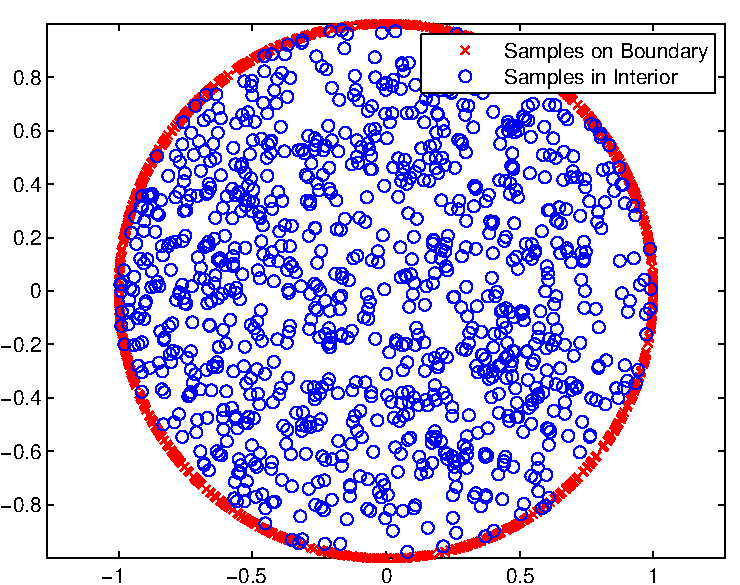
\includegraphics[width=4in]{figs/psamplePLOT.pdf}
\caption{Samples on the boundary and in the interior of a unit disk
obtained with \texttt{psample}}
\end{center}
\end{figure}


%------------------------------------------------------------------------
\newpage
\subsection{PSIM}
\begin{verbatim}
function [xtraj,xconv]=psim(f,x,x0,tfinal,event_params,opts)

  DESCRIPTION
    Simulates non-autonomous polynomial systems of the form:
                dx/dt = f(x),   x(t) = x0

  INPUTS
    f: Vector field  (Ns-by-1 polynomial)
    x: State  (Ns-by-1 vector of pvars)
    x0: Initial Conditions (Ns-by-N0 array of doubles)
    tfinal: Final simulation time unless the simulation is terminated
      by one of the event parameters  (scalar)
    event_params (Optional):  Event parameters for stopping the
      simulation.  This is a structure with the following fields:
       *nbig: Terminate if norm(x) is greater than nbig*norm(x0)
       *nsmall: Terminate if norm(x) is less than nsmall*norm(x0)
       *xbig: Terminate if any abs(x(i)) is greater than xbig(i)
       *xsmall: Terminate if all abs(x(i)) are less than xsmall(i)
       *funchandle:  Handle to a user specified event function.
       *Additional fields can be used to pass parameter data to the
           user defined event function
       (Default: nbig = 1e6, nsmall = 1e-6, xbig =0, xsmall=0,
           funchandle = [])
    opts (Optional): Options structure passed to ODE solver. See
        odeset and odeget for more details.  opts can have the additonal
        field 'Solver' to specify the ode solver.  The 'Solver' field
        can be ode45 or ode15s.

  OUTPUTS
    xtraj: N0-by-2 cell array with the i^th row containing the simulation
       results starting from x0(:,i).  xtraj{i,1} is an Nt-by-1 vector
       of simulation times and xtraj{i,2} is an Nt-by-Ns matrix of
       the state trajectories.
    xconv: N0-by-1 logical vector with the i^th element = 1 if the
       corresponding trajectory converged to the origin and = 0 otherwise.
       A trajectory is considered to have converged to the origin if
       either the nsmall or xsmall event occured.

  SYNTAX
    [xtraj,xconv]=psim(f,x,x0,tfinal)
    [xtraj,xconv]=psim(f,x,x0,tfinal,event_params)
    [xtraj,xconv]=psim(f,x,x0,tfinal,event_params,opts)

  See also:
   ODE solvers: ode45, ode23, ode113, ode15s, ode23s, ode23t, ode23tb
   Options handling: odeset, odeget

\end{verbatim}

%------------------------------------------------------------------------
\newpage
\subsection{PPLANESIM}
\begin{verbatim}
function  [Xsimdata] = pplanesim(f,x,figno,x0,psimopts)

  DESCRIPTION
    Draws the phase plane for a non-autonomous polynomial system:
                dx/dt = f(x),   x(t) = x0

  INPUTS:
    f: Vector field  (2-by-1 polynomial or function handle)
    x: State  (2-by-1 vector of pvars
    figno: Figure number for plotting
    x0: 2-by-Npts array of initial conditions. Alternatively, the initial
       conditions options can be specified as a structure with fields:
       - range: 2-by-2 matrix with the i^th row specifying the min and
         max value of the i^th state. default is [-1 1; -1 1]
       - Npts: Number of initial conditions.  The actual number of points
         depends on the sampling type (see sample below). (default is 100)
       - conv: True to plot only convergent trajectories (Default is false)
       - div: True to plot only divergent trajectories (Default is false)
       - sample: Sampling technique to be specified.  Choices are:
          - 'grid': Generates ceil(sqrt(Npts)) points linearly spaced
             along each direction.
          - 'bndry': Samples ceil(Npts/4) points along each of the
             boundary specified by range.
     psimopts:  Options structure passed to ODE solver.

  OUTPUTS:
     if no argument is invoked then only plot will be generated. However,
     if one argument is invoked, then it will also return the simulation data.
     For more information on the output refer to psim. The two outputs xtraj and
     xconv will be bundled in the output argument as a cell array object.

  SYNTAX
   pplanesim(f,x,figno,x0,psimopts)
     Generate phase plane plot
   Xsimdata = pplanesim(f,x,figno,x0,psimopts)
     Output all simulation data.

\end{verbatim}


%------------------------------------------------------------------------
\newpage
\subsection{INT}
\begin{verbatim}

function B = int(A,X,L,U)

  DESCRIPTION
    Element-by-element integration of a polynomial with respect
    to a single variable.

  INPUTS
    A: polynomial
    X: Scalar polynomial variable [Optional with default X = A.varname{1}]
    L: Lower limit of definite integral
    U: Upper limit of definite integral

  OUTPUTS
    B: polynomial

  SYNTAX
    B = int(A,X)
      Indefinite integral of the polynomial, A, with respect to X.
      X should be a polynomial variable or string.   Integration is done
      element-by-element if A is a matrix.
    B = int(A,X,L,U)
      Definite integral of A with respect to X from lower limit L to
      upper limit U.
    B = int(A,X,[L U]);
      Equivalent to B = diff(A,X,L,U)

  EXAMPLE
    pvar x y z;
    a = 2*x^3 - 2*x*z^2 + 5*y*z;
    b = int(a,x)
b =
  0.5*x^4 - x^2*z^2 + 5*x*y*z

    diff(b,x)-a
ans =
  0

    c = int(a,[0 1])
c =
  5*y*z - z^2 + 0.5

  See also: diff, jacobian

\end{verbatim}

%------------------------------------------------------------------------
\newpage
\subsection{DIFF}
\begin{verbatim}
function B=diff(A,X)

  DESCRIPTION
    Element-by-element differentiation of a polynomial with respect
    to a single variable.

  INPUTS
    A: polynomial
    X: Differentiate with respect to the (single) variable X.

  OUTPUTS
    B: polynomial

  SYNTAX
    B = diff(A,X);
      Differentiate the polynomial, A, with to X.  A should be a
      polynomial and X should be a polynomial variable or a string.
      Differentiation is done element-by-element if A is a matrix.

  EXAMPLE
    pvar x y z;
    f = 2*x^3+5*y*z-2*x*z^2;
    df = diff(f,x)
df =
  6*x^2 - 2*z^2

  See also: jacobian

\end{verbatim}

%------------------------------------------------------------------------
\newpage
\subsection{JACOBIAN}
\begin{verbatim}
function J = jacobian(F,X)

  DESCRIPTION
    Compute the Jacobian matrix. The (i,j)-th entry of J is dF(i)/dX(j).

  INPUTS
    F: Polynomial to differentiate (N-by-1 polynomial)
    X: Variable for differentiation (V-by-1 vector of pvars
         or cell array of strings)

  OUTPUTS
    J: Jacobian of F with respect to X (N-by-V polynomial)

  SYNTAX
    J = jacobian(F);
      Computes the Jacobian of F with respect to F.varname
    J = jacobian(F,X);
      Computes the Jacobian of F with respect to X

  EXAMPLE
    pvar x y z;
    f = [x^3+5*y*z; 2*x*z; 3*x+4*y+6*z];
    J = jacobian(f,[x;y;z])
J =
  [ 3*x^2, 5*z, 5*y]
  [   2*z,   0, 2*x]
  [     3,   4,   6]

  See also: diff

\end{verbatim}


%------------------------------------------------------------------------
\newpage
\subsection{COLLECT}
\begin{verbatim}
function [g0,g,h] = collect(p,x);

  DESCRIPTION
    Collect p(x,y) into the form g0(x)+g(x)*h(y) where h(y) is a vector
    of unique monomials in y.

  INPUTS
    p: M-by-1 polynomial in variables x and y.
    x: variables of p to collect into polynomials with coefficients given
       by monomials in y. x can either be a polynomial vector or
       a cell array of strings of variable names.

  OUTPUTS
    g0: M-by-1 polynomial in x.
    g: M-by-N vector of polynomials in x.
    h: N-by-1 vector of monomials in y.

  SYNTAX
    [g0,g,h] = collect(p,x);
       g0, g, and h satisfy p(x,y) = g0(x)+ g(x)*h(y)

  EXAMPLE
    pvar x1 x2 y1 y2;
    p = 13+x1^2*y1-5*x1^2*y2^3+6*x1*x2*y1+8*x1;
    x = [x1;x2];
    [g0,g,h] = collect(p,x)
g0 =
  8*x1 + 13
g =
  [ x1^2 + 6*x1*x2, -5*x1^2]
h =
  [   y1]
  [ y2^3]

    p-(g0+g*h)
ans =
  0
\end{verbatim}

%------------------------------------------------------------------------
\newpage
\subsection{SUBS}
\begin{verbatim}
 function B = subs(A,Old,New);

  DESCRIPTION
   Symbolic Substitution.

  INPUTS
    A: Nr-by-Nc polynomial array
    Old: No-by-1 array of polynomial variables or No-by-1 cell array
        of characters. The entries of Old must be unique.
    New: No-by-Npts array of polynomials or doubles.  If Npts>1 then
        A must be a column or row vector.

  OUTPUTS
    B:  polynomial. B is always returned as a polynomial. Use 'double'
        to convert B to a double when the final result is a constant.
        If Npts=1 then B is Nr-by-Nc.  If Npts>1, B is Nr-by-Npts when
        Nc=1 and Npts-by-Nc otherwise.

  SYNTAX
    B = subs(A,Old,New);
      Replaces variables in Old with the corresponding entries in New.
    B = subs(A);
      Replaces all variables in A with values in the BASE workspace.
    B = subs(A,New);
      If New is an 1-by-1 polynomial array then this is equivalent
      B=subs(A,A.varname{1},New).  Otherwise, this is equivalent to
      B=subs(A,New(:,1),New(:,2:end)).

  EXAMPLE
   pvar x1 x2 y
   x=[x1;x2];
   p=2*(x1+x2)^2+5;
   subs(p,x,[1;2])
ans =
  23

   subs(p,x,[0 1 1; 1 0 2])
ans =
  [ 7, 7, 23]

   subs(p,x1,y)
ans =
  2*x2^2 + 4*x2*y + 2*y^2 + 5

  See also double

\end{verbatim}

%------------------------------------------------------------------------
\newpage
\subsection{CLEANPOLY}
\begin{verbatim}
function B = cleanpoly(A,tol,deg)

  DESCRIPTION
    Cleans up the input polynomial.  The output polynomial includes only
    terms whose coefficients have magnitude greater than or equal to TOL
    and whose monomial degree is specified by DEG.

  INPUTS
    A: polynomial
    tol: scalar double specifying the coefficient tolerance
    deg: vector of non-negative integers specifying the degrees of
         mononmials to retain. Alternatively deg can be an N-by-2
         cell array with deg{i,1} specifying a variable and
         deg{i,2} specifying a vector of non-negative integers.
         This will retain only monomials whose degree in variable
         deg{i,1} is specified in deg{i,2}.

  OUTPUTS
    B: polynomial which only contains the terms of A whose coefficients
       have magnitude greater than or equal to tol and whose monomial
       degree is listed in deg.

  SYNTAX
    B=cleanpoly(A,tol);
    B=cleanpoly(A,[],deg);
    B=cleanpoly(A,tol,deg);

  EXAMPLE
    pvar x1 x2 u;
    p = 9*u^3 + u*x1^2 + 1e-6*u^2*x1*x2 + 1e-5*u*x2^2 + 2*x1^3 ...
         - x1*x2 + 3*u + x1 + 2*x2;

    % Remove terms whose coefficients has magnitude < tol
    tol = 1e-4;
    p1 = cleanpoly(p,tol)
p1 =
  9*u^3 + u*x1^2 + 2*x1^3 - x1*x2 + 3*u + x1 + 2*x2

    % Retain linear and quadratic terms
    p2 = cleanpoly(p,[],1:2)
p2 =
  -x1*x2 + 3*u + x1 + 2*x2

    % Retain terms linear in u but of degree 0,1,2,3 in x1 and x2
    p3 = cleanpoly(p,[],{x1, 0:3; x2, 0:3; u 1})
p3 =
  u*x1^2 + 1e-005*u*x2^2 + 3*u

\end{verbatim}

%------------------------------------------------------------------------
\newpage
\subsection{P2S}
\begin{verbatim}
 function s=p2s(p)

 DESCRIPTION
   Converts from a multipoly polynomial to a symbolic math toolbox polynomial.

 INPUTS
   p: Polynomial created using the multipoly toolbox

 OUTPUTS
   s: Polynomial created using the symbolic math toolbox

 SYNTAX
   s = p2s(p)

 See also s2p
\end{verbatim}
%------------------------------------------------------------------------
\newpage
\subsection{S2P}
\begin{verbatim}
 function p=s2p(s)

 DESCRIPTION
   Converts from a symbolic math toolbox polynomial to a multipoly polynomial.

 INPUTS
   s: Polynomial created using the symbolic math toolbox

 OUTPUTS
   p: Polynomial created using the multipoly toolbox

 SYNTAX
   p = s2p(s)

 See also p2s
\end{verbatim}


\end{document}







